\problem{Laplace Transforms and Symbolic Math Toolbox (Project 5)}

This homework focuses on the following function: 
$$ Y(s) = \frac{4s^2 + 4s + 4}{s^2 * (s^2 + 3s + 2)} $$

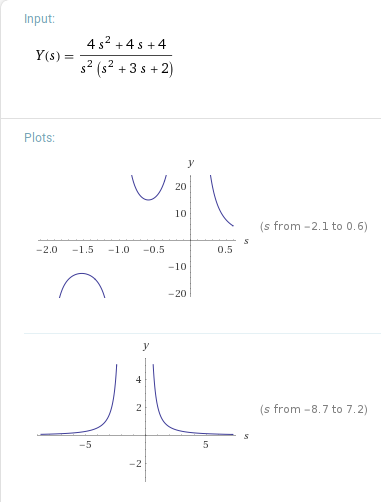
\includegraphics[scale=0.7]{1.png}

\solution

This project asks for the following:
\begin{enumerate}
    \item Residues and poles of $Y(s)$, and the partial fraction decomposition, which is $\frac{2}{s^2} + \frac{4}{s + 1} + \frac{3}{s + 2} + \frac{1}{s}$.
    \item The Inverse Laplace Transform of $Y(s)$ from a table, which is $2t - 3e^{-2t} + 4e^{-t} - 1$.
    \item Checking the Laplace Transform of $Y(s)$ by taking a computational Inverse Laplace Transform, which also gives $2t - 3e^{-2t} + 4e^{-t} - 1$ (equivalently).
\end{enumerate}
